%% This is file `elsarticle-template-1-num.tex',
%%
%% Copyright 2009 Elsevier Ltd
%%
%% This file is part of the 'Elsarticle Bundle'.
%% ---------------------------------------------
%%
%% It may be distributed under the conditions of the LaTeX Project Public
%% License, either version 1.2 of this license or (at your option) any
%% later version.  The latest version of this license is in
%%    http://www.latex-project.org/lppl.txt
%% and version 1.2 or later is part of all distributions of LaTeX
%% version 1999/12/01 or later.
%%
%% Template article for Elsevier's document class `elsarticle'
%% with numbered style bibliographic references
%%
%% $Id: elsarticle-template-1-num.tex 149 2009-10-08 05:01:15Z rishi $
%% $URL: http://lenova.river-valley.com/svn/elsbst/trunk/elsarticle-template-1-num.tex $
%%
\documentclass[final,12pt,a4paper]{elsarticle}

%% Use the option review to obtain double line spacing
%% \documentclass[preprint,review,12pt]{elsarticle}

%% Use the options 1p,twocolumn; 3p; 3p,twocolumn; 5p; or 5p,twocolumn
%% for a journal layout:
%% \documentclass[final,1p,times]{elsarticle}
%% \documentclass[final,1p,times,twocolumn]{elsarticle}
%% \documentclass[final,3p,times]{elsarticle}
%% \documentclass[final,3p,times,twocolumn]{elsarticle}
%% \documentclass[final,5p,times]{elsarticle}
%% \documentclass[final,5p,times,twocolumn]{elsarticle}

%% The graphicx package provides the includegraphics command.
\usepackage{graphicx}
%% The amssymb package provides various useful mathematical symbols
\usepackage{amssymb}
%% The amsthm package provides extended theorem environments
%% \usepackage{amsthm}

\usepackage[margin=2cm]{geometry}
\usepackage{booktabs}
\usepackage{xcolor}
\usepackage{sourcecodepro}
\usepackage{url}
\usepackage{listings}
\usepackage[utf8]{inputenc}
\usepackage[brazilian]{babel}
\usepackage{multirow}
\usepackage{textcomp}
\usepackage{caption}

\definecolor{Accent}{HTML}{bb0300}

\lstdefinestyle{customMtheme}{%
  backgroundcolor={},
  basicstyle=\ttfamily\scriptsize,
  breakatwhitespace=true,
  breaklines=true,
  captionpos=n,
  commentstyle=\color{orange},
  escapeinside={\%*}{*)},
  extendedchars=true,
  frame=n,
  keywordstyle=\color{Accent},
  language=C++,
  rulecolor=\color{black},
  showspaces=false,
  showstringspaces=false,
  xleftmargin=.5cm,
  xrightmargin=.5cm,
  showtabs=false,
  stepnumber=2,
  stringstyle=\color{gray},
  tabsize=4,
  keywords={void, int, float, main,
  if, else, malloc, NULL,
  fprintf, stderr, for, make, gcc, o, Enter, Ctrl},
  otherkeywords={\#pragma, \#include, \&, \*, +, -, /, [, ], >, <, \$, \., std\=c11}
}
\lstset{basicstyle=\ttfamily\scriptsize,style=customMtheme}

\renewcommand*{\UrlFont}{\ttfamily\scriptsize\relax}

\graphicspath{{./img/}}

%% The lineno packages adds line numbers. Start line numbering with
%% \begin{linenumbers}, end it with \end{linenumbers}. Or switch it on
%% for the whole article with \linenumbers after \end{frontmatter}.
%% \usepackage{lineno}

%% natbib.sty is loaded by default. However, natbib options can be
%% provided with \biboptions{...} command. Following options are
%% valid:

%%   round  -  round parentheses are used (default)
%%   square -  square brackets are used   [option]
%%   curly  -  curly braces are used      {option}
%%   angle  -  angle brackets are used    <option>
%%   semicolon  -  multiple citations separated by semi-colon
%%   colon  - same as semicolon, an earlier confusion
%%   comma  -  separated by comma
%%   numbers-  selects numerical citations
%%   super  -  numerical citations as superscripts
%%   sort   -  sorts multiple citations according to order in ref. list
%%   sort&compress   -  like sort, but also compresses numerical citations
%%   compress - compresses without sorting
%%
%% \biboptions{comma,round}

% \biboptions{}

%% Removing lines when no abstract is given
\makeatletter
\renewcommand{\MaketitleBox}{%
    \resetTitleCounters
        \def\baselinestretch{1}%
        \begin{center}
    \def\baselinestretch{1}%
        \Large \@title \par
        \vskip 18pt
        \normalsize\elsauthors \par
        \vskip 10pt
        \footnotesize \itshape \elsaddress \par
        \end{center}
    \vskip 12pt
}
\makeatother

%% Removing custom footer on fist page
\makeatletter
\def\ps@pprintTitle{%
    \let\@oddhead\@empty
        \let\@evenhead\@empty
        \def\@oddfoot{\centerline{\thepage}%
        }%
    \let\@evenfoot\@oddfoot
}%
\makeatother

\journal{MAC 5742-0219 Introdução à Programação Concorrente, Paralela e Distribuída}

\begin{document}

\begin{frontmatter}

%% Title, authors and addresses

\title{EP1: Cálculo do Conjunto de Mandelbrot \\ em Paralelo com Pthreads e OpenMP}

%% use the tnoteref command within \title for footnotes;
%% use the tnotetext command for the associated footnote;
%% use the fnref command within \author or \address for footnotes;
%% use the fntext command for the associated footnote;
%% use the corref command within \author for corresponding author footnotes;
%% use the cortext command for the associated footnote;
%% use the ead command for the email address,
%% and the form \ead[url] for the home page:
%%
%% \title{Title\tnoteref{label1}}
%% \tnotetext[label1]{}
%% \author{Name\corref{cor1}\fnref{label2}}
%% \ead{email address}
%% \ead[url]{home page}
%% \fntext[label2]{}
%% \cortext[cor1]{}
%% \address{Address\fnref{label3}}
%% \fntext[label3]{}


%% use optional labels to link authors explicitly to addresses:
%% \author[label1,label2]{<author name>}
%% \address[label1]{<address>}
%% \address[label2]{<address>}

\author{Pedro Bruel, Anderson Andrei, e Alfredo Goldman}

\address{MAC 5742-0219 Introdução à Programação Concorrente, Paralela e Distribuída}

%%\begin{abstract}
%% Text of abstract
%% Suspendisse potenti. Suspendisse quis sem elit, et mattis nisl. Phasellus
%% consequat erat eu velit rhoncus non pharetra neque auctor. Phasellus eu lacus
%% quam. Ut ipsum dolor, euismod aliquam congue sed, lobortis et orci. Mauris eget
%% velit id arcu ultricies auctor in eget dolor. Pellentesque suscipit adipiscing
%% sem, imperdiet laoreet dolor elementum ut. Mauris condimentum est sed velit
%% lacinia placerat. Vestibulum ante ipsum primis in faucibus orci luctus et
%% ultrices posuere cubilia Curae; Nullam diam metus, pharetra vitae euismod sed,
%% placerat ultrices eros. Aliquam tincidunt dapibus venenatis. In interdum tellus
%% nec justo accumsan aliquam. Nulla sit amet massa augue.
%% \end{abstract}
%%
%% \begin{keyword}
%% Science \sep Publication \sep Complicated
%% keywords here, in the form: keyword \sep keyword

%% MSC codes here, in the form: \MSC code \sep code
%% or \MSC[2008] code \sep code (2000 is the default)

%% \end{keyword}

\end{frontmatter}

%%
%% Start line numbering here if you want
%%
%% \linenumbers

%% main text
\section{Introdução}

Você já ouviu falar do Conjunto de
Mandelbrot\footnote{\url{https://en.wikipedia.org/wiki/Mandelbrot_set}
[Acessado em 24/04/2020]}?  Seu descobridor foi Benoit Mandelbrot, que
trabalhava na IBM durante a década de 1960 e foi um dos primeiros a usar
computação gráfica para mostrar como complexidade pode surgir a partir de
regras simples. Benoit fez isso gerando e visualizando imagens de geometria
fractal.

Um desses fractais  foi nomeado \textit{Conjunto de  Mandelbrot} pelo matemático
Adrien Douady.  O Conjunto de Mandelbrot  pode ser informalmente definido como o
conjunto dos números complexos $c$ para os quais a função $f_c(z) = z^2 + x$ não
diverge quando  é iterada  começando em $z  = 0$. Isto  é, a  sequência $f_c(0),
f_c(f_c(0)),    f_c(f_c(f_c(0))),\dots$   é    sempre    limitada.   A    Figura
\ref{fig:header}  mostra uma  região do  Conjunto de  Mandelbrot conhecida  como
\textit{Seahorse Valley}.

\begin{figure}[htpb]
    \centering
    
\includegraphics[width=.82\textwidth]{seahorse}
    \caption{Seahorse Valley}
    \label{fig:header}
\end{figure}

As cores na Figura \ref{fig:header} indicam o número da iteração onde a
função $f_c(z)$ convergiu. A Figura \ref{fig:header} foi gerada usando o
código fonte fornecido junto com este documento. O código na linguagem
\texttt{C} e os arquivos em \LaTeX{} necessários para gerar este documento
estão disponíveis no
\textit{GitHub}\footnote{\url{https://github.com/phrb/MAC5742-0219-EP1}
[Acessado em 27/04/2020]}. O resto deste documento descreve as tarefas que você
e seu grupo deverão realizar no EP1.

\section{Tarefas}

Você e seu grupo deverão paralelizar o código para o cálculo do Conjunto de
Mandelbrot usando a biblioteca Pthreads e as diretivas de compilador fornecidas
pelo OpenMP. Depois, vocês deverão medir o tempo de execução das versões
sequencial, paralelizada com Pthreads e paralelizada com OpenMP. Vocês deverão
medir o tempo de execução para diferentes tamanhos de entrada e números de
\textit{threads} nas versões paralelizadas, em quatro regiões do Conjunto
de Mandelbrot.

A implementação necessária para paralelizar o código fornecido usando Pthreads e
OpenMP é relativamente simples. A parte mais trabalhosa do EP1 é a elaboração de
um relatório, no formato \textit{Jupyter Notebook} usando a linguagem Julia, que
apresente gráficos com os resultados obtidos com as paralelizações, e os discuta
de forma metódica, como vocês fizeram nos miniEPs.

\subsection{Paralelização com Pthreads e OpenMP}

O código fornecido está triplicado, e cada arquivo \texttt{.c}
tem um propósito diferente:

\begin{itemize}
    \item \texttt{mandelbrot\_seq.c}: não precisa ser paralelizado
    \item \texttt{mandelbrot\_omp.c}: deve ser paralelizado com OpenMP
    \item \texttt{mandelbrot\_pth.c}: deve ser paralelizado com Pthreads
\end{itemize}

Vocês  podem  modificar  à  vontade  os  arquivos  \texttt{mandelbrot\_omp.c}  e
\texttt{mandelbrot\_pth.c}, desde  que eles  continuem produzindo a  mesma saída
produzida por \texttt{mandelbrot\_seq.c}. Vocês também podem modificar o arquivo
sequencial, dado que a saída continue correta.

\subsection{Experimentos}

Para cada uma  das três versões do programa, vocês  deverão realizar medições do
tempo de execução para diferentes tamanhos de entrada. Nas versões paralelizadas
vocês deverão  também medir, para cada  tamanho de entrada, o  tempo de execução
para diferentes números de \textit{threads}.

Vocês  devem fazer  um número  de  medições e  analisar a  variação dos  valores
obtidos.  Sugerimos $10$ medições para cada experimento, e também que vocês usem
a média e  o intervalo de confiança  das $10$ medições nos  seus gráficos. Vocês
podem  fazer mais  medições,  desde que  apresentem  a média  e  o intervalo  de
confiança.  \textbf{Não é recomendado} fazer menos de $10$ medições.

Vocês devem analisar  também o impacto das porções não  paralelizáveis do código
sequencial:  as operações  de  I/O e  alocação  de memória.   Uma  vez que  você
verifique  que  as versões  paralelizadas  produzem  o resultado  correto,  elas
\textbf{não  precisam}  realizar  I/O  e  alocação  de  memória  nos  testes  de
desempenho, pois esses custos são fixos e assim aceleramos os experimentos.

A Tabela  \ref{tab:exp} lista os experimentos  que devem ser feitos:  os valores
para o  número de  \textit{threads} e  de execuções, e  os tamanhos  de entrada.
Cada  experimento  deverá  ser  repetido nas  quatro  regiões  especificadas  na
Figura~\ref{fig:regions}.  As coordenadas  para  cada região  podem ser  obtidas
executando no diretório \texttt{src}:

\begin{lstlisting}
$ make mandelbrot_seq
gcc -o mandelbrot_seq -std=c11 mandelbrot_seq.c
$ ./mandelbrot_seq
usage: ./mandelbrot_seq c_x_min c_x_max c_y_min c_y_max image_size
examples with image_size = 11500:
    Full Picture:         ./mandelbrot_seq -2.5 1.5 -2.0 2.0 11500
    Seahorse Valley:      ./mandelbrot_seq -0.8 -0.7 0.05 0.15 11500
    Elephant Valley:      ./mandelbrot_seq 0.175 0.375 -0.1 0.1 11500
    Triple Spiral Valley: ./mandelbrot_seq -0.188 -0.012 0.554 0.754 11500
\end{lstlisting}

O número de iterações para o critério de convergência foi
escolhido\footnote{\url{https://goo.gl/WpL9hS} [Acessado em 27/04/2020]} de
forma a produzir uma imagem interessante em diferentes níveis de magnificação,
mas ter um tempo de execução razoável para tamanhos grandes de entrada.

\begin{figure}[htpb]
    \captionsetup{width=.4\linewidth}
    \centering
    \begin{minipage}{.48\textwidth}
    \centering
        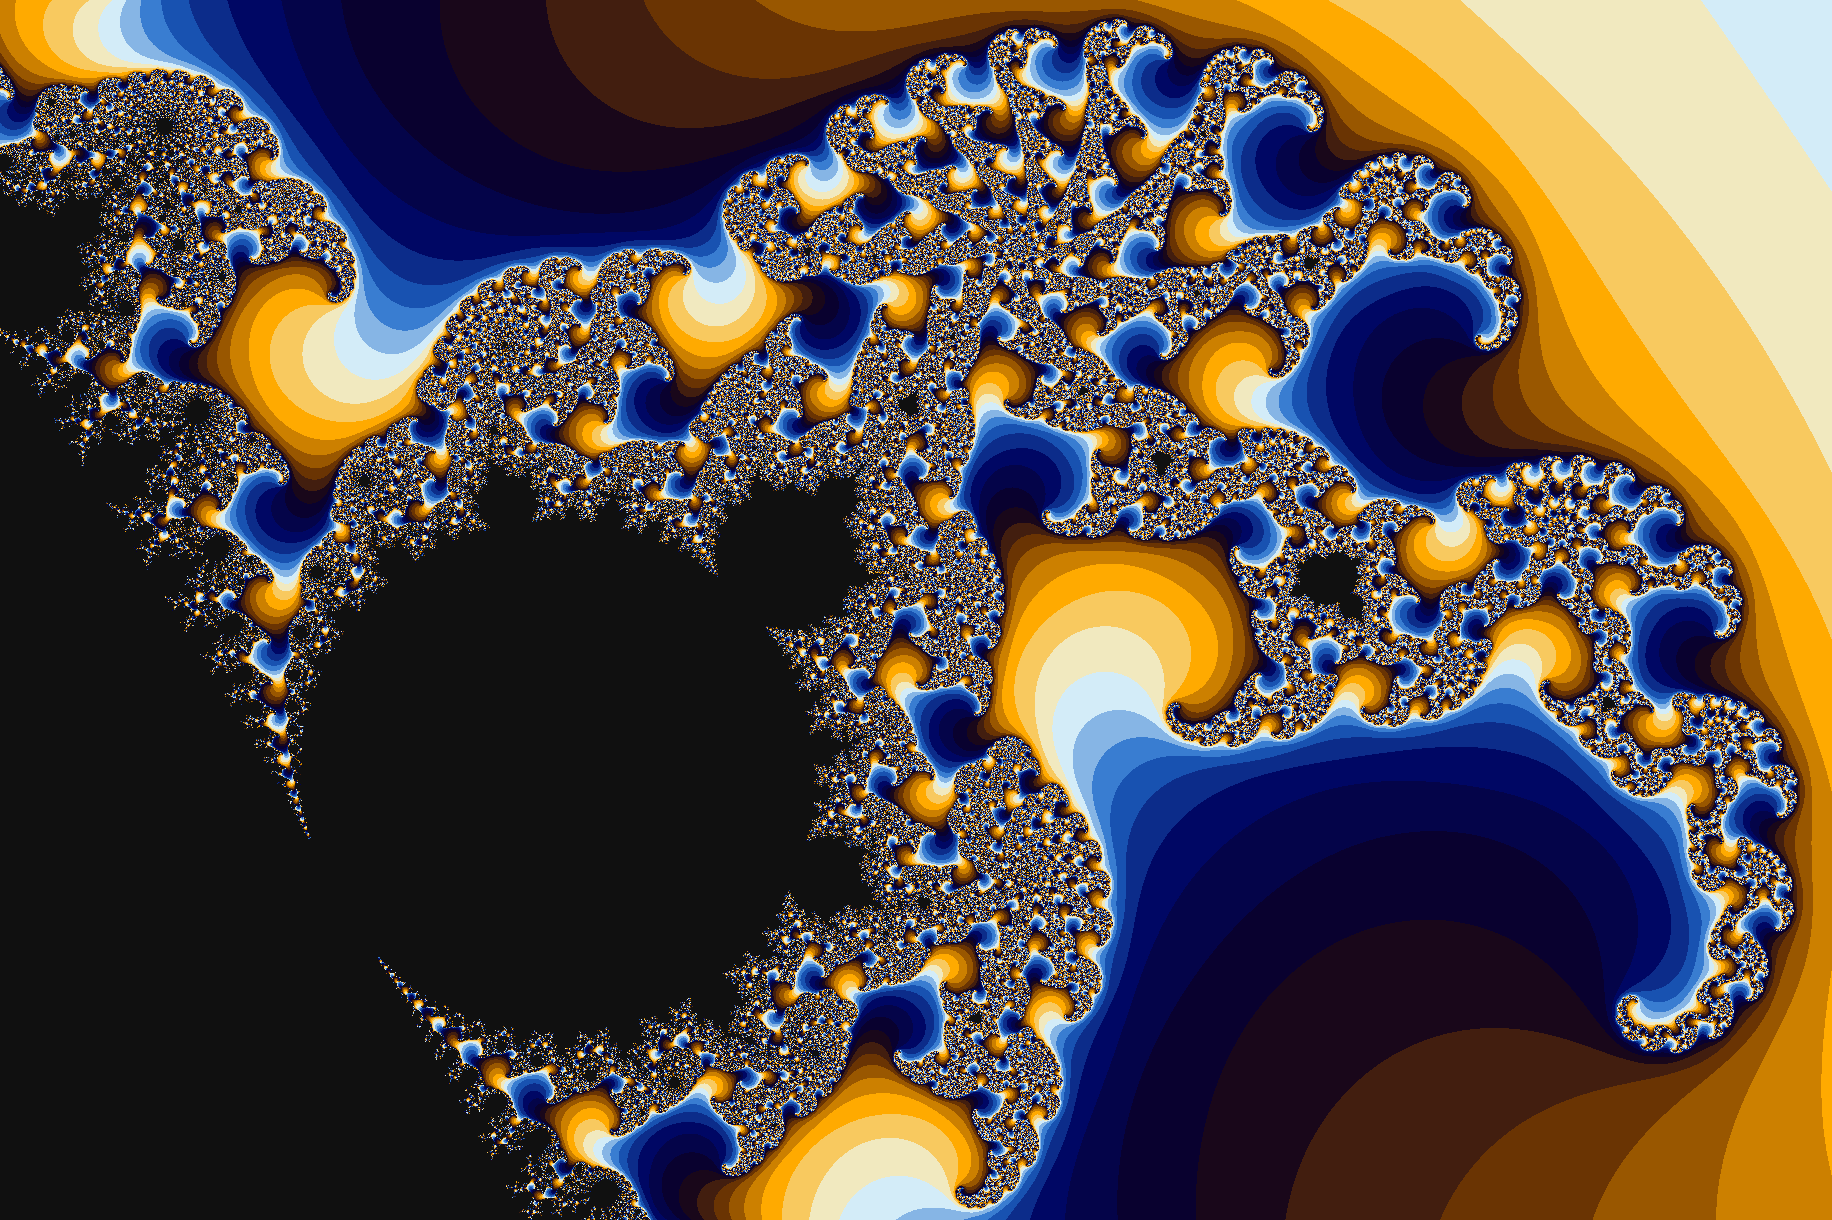
\includegraphics[width=.95\textwidth]{elephant}
    \caption{\textit{Elephant Valley}}
    \label{fig:regions}
    \end{minipage}%
    \begin{minipage}{.48\textwidth}
    \centering
        
\includegraphics[width=.95\textwidth]{seahorse}
    \caption{\textit{Seahorse Valley}}
    \label{fig:regions}
    \end{minipage}

    \begin{minipage}{.48\textwidth}
    \centering
        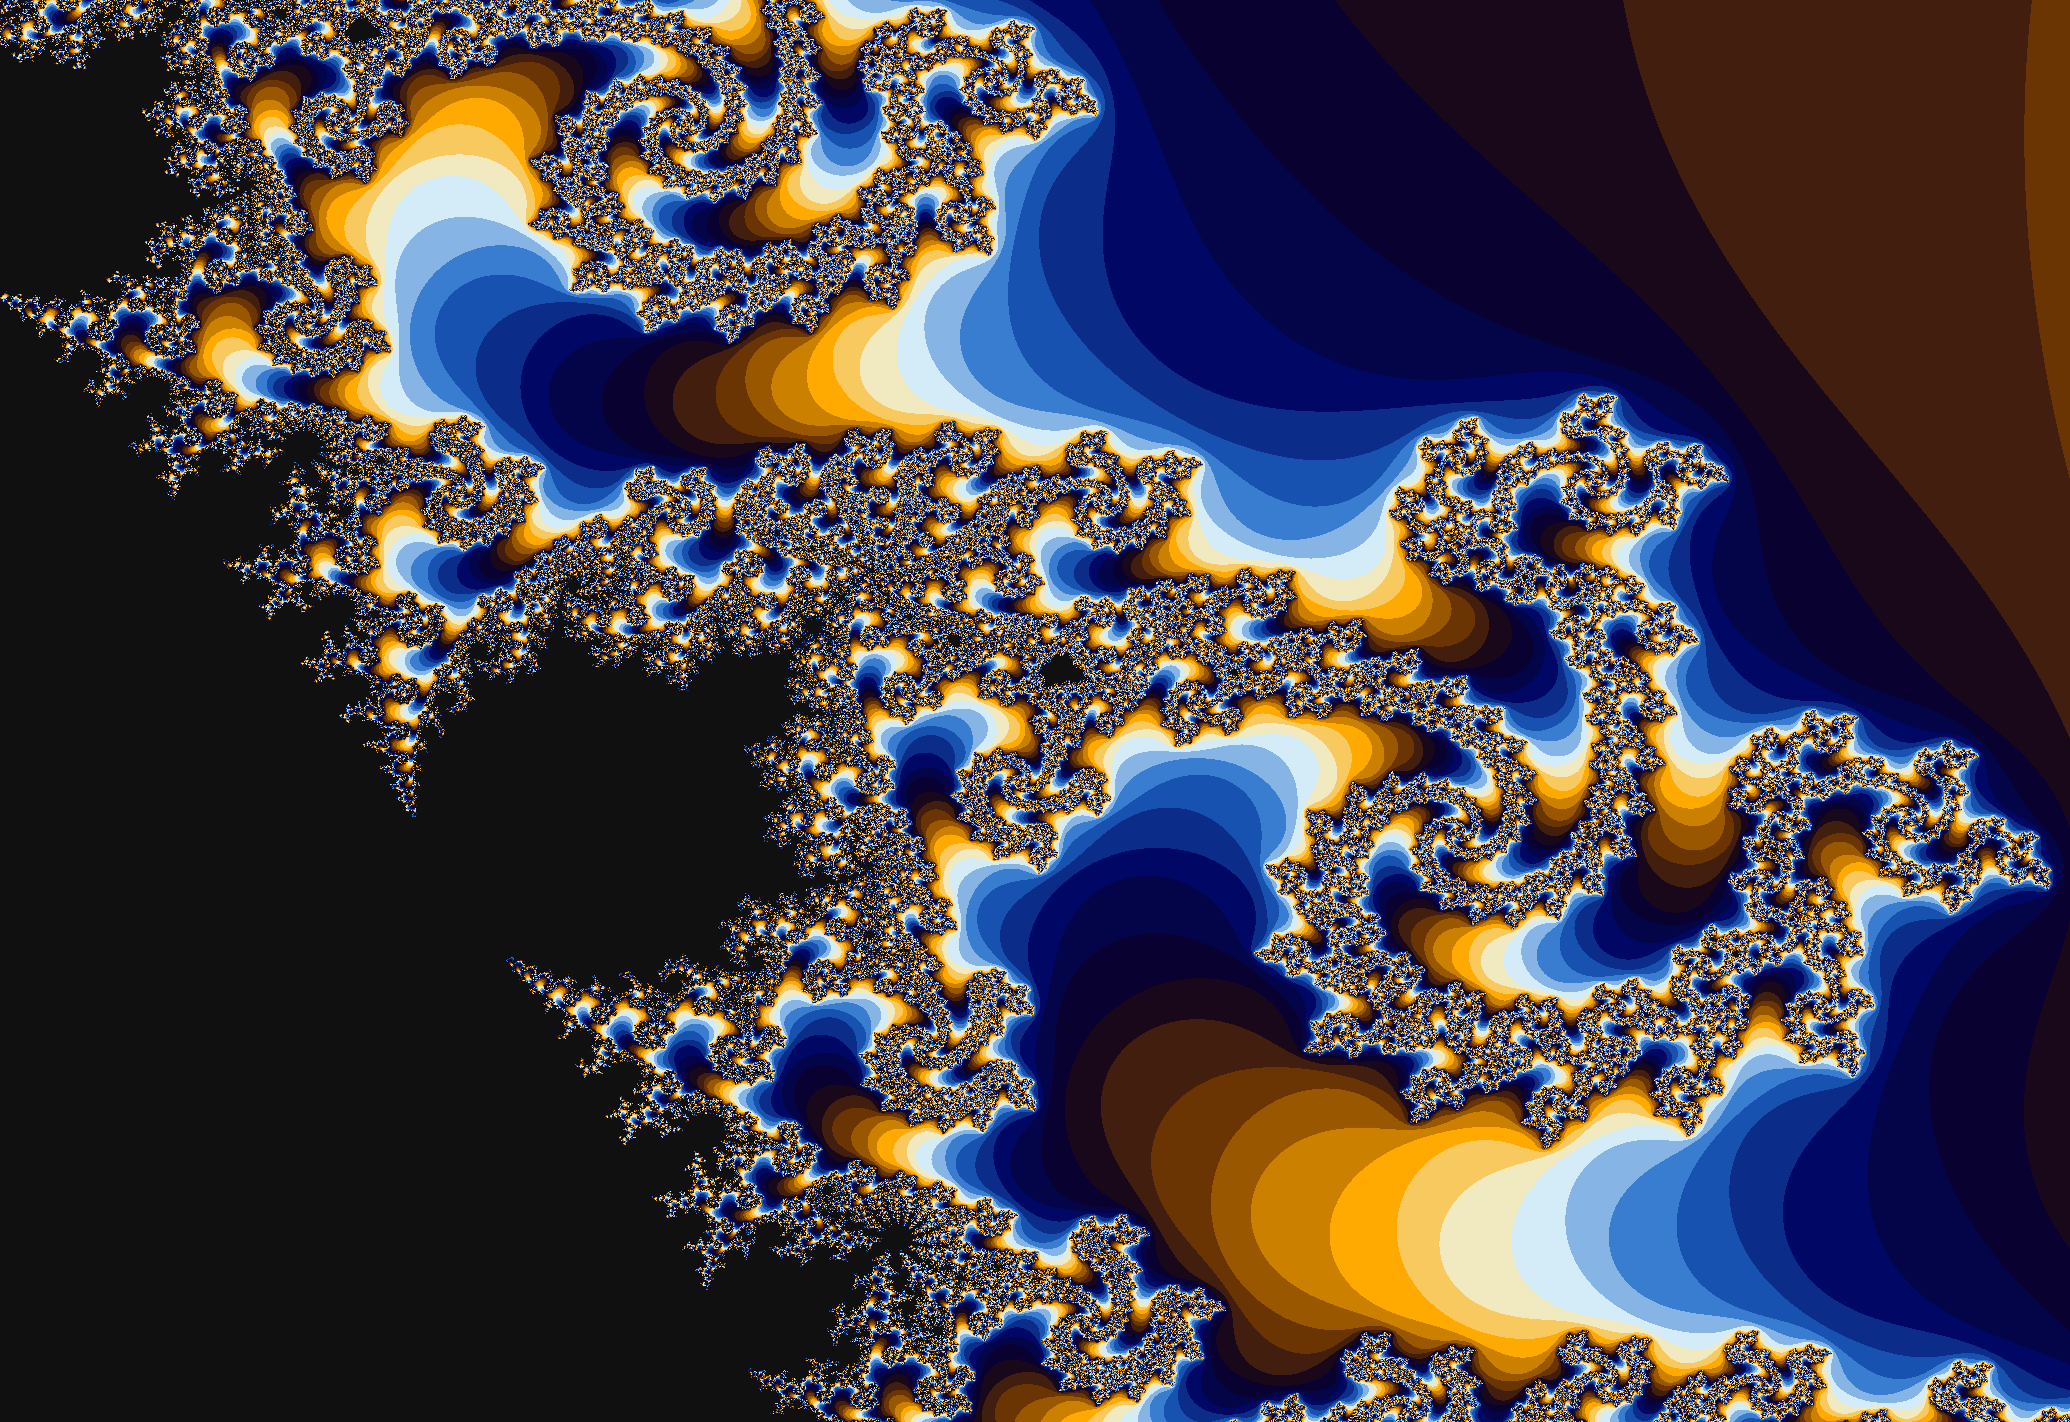
\includegraphics[width=.95\textwidth]{triple_spiral}
    \caption{\textit{Triple Spiral Valley}}
    \label{fig:regions}
    \end{minipage}%
    \begin{minipage}{.48\textwidth}
    \centering
        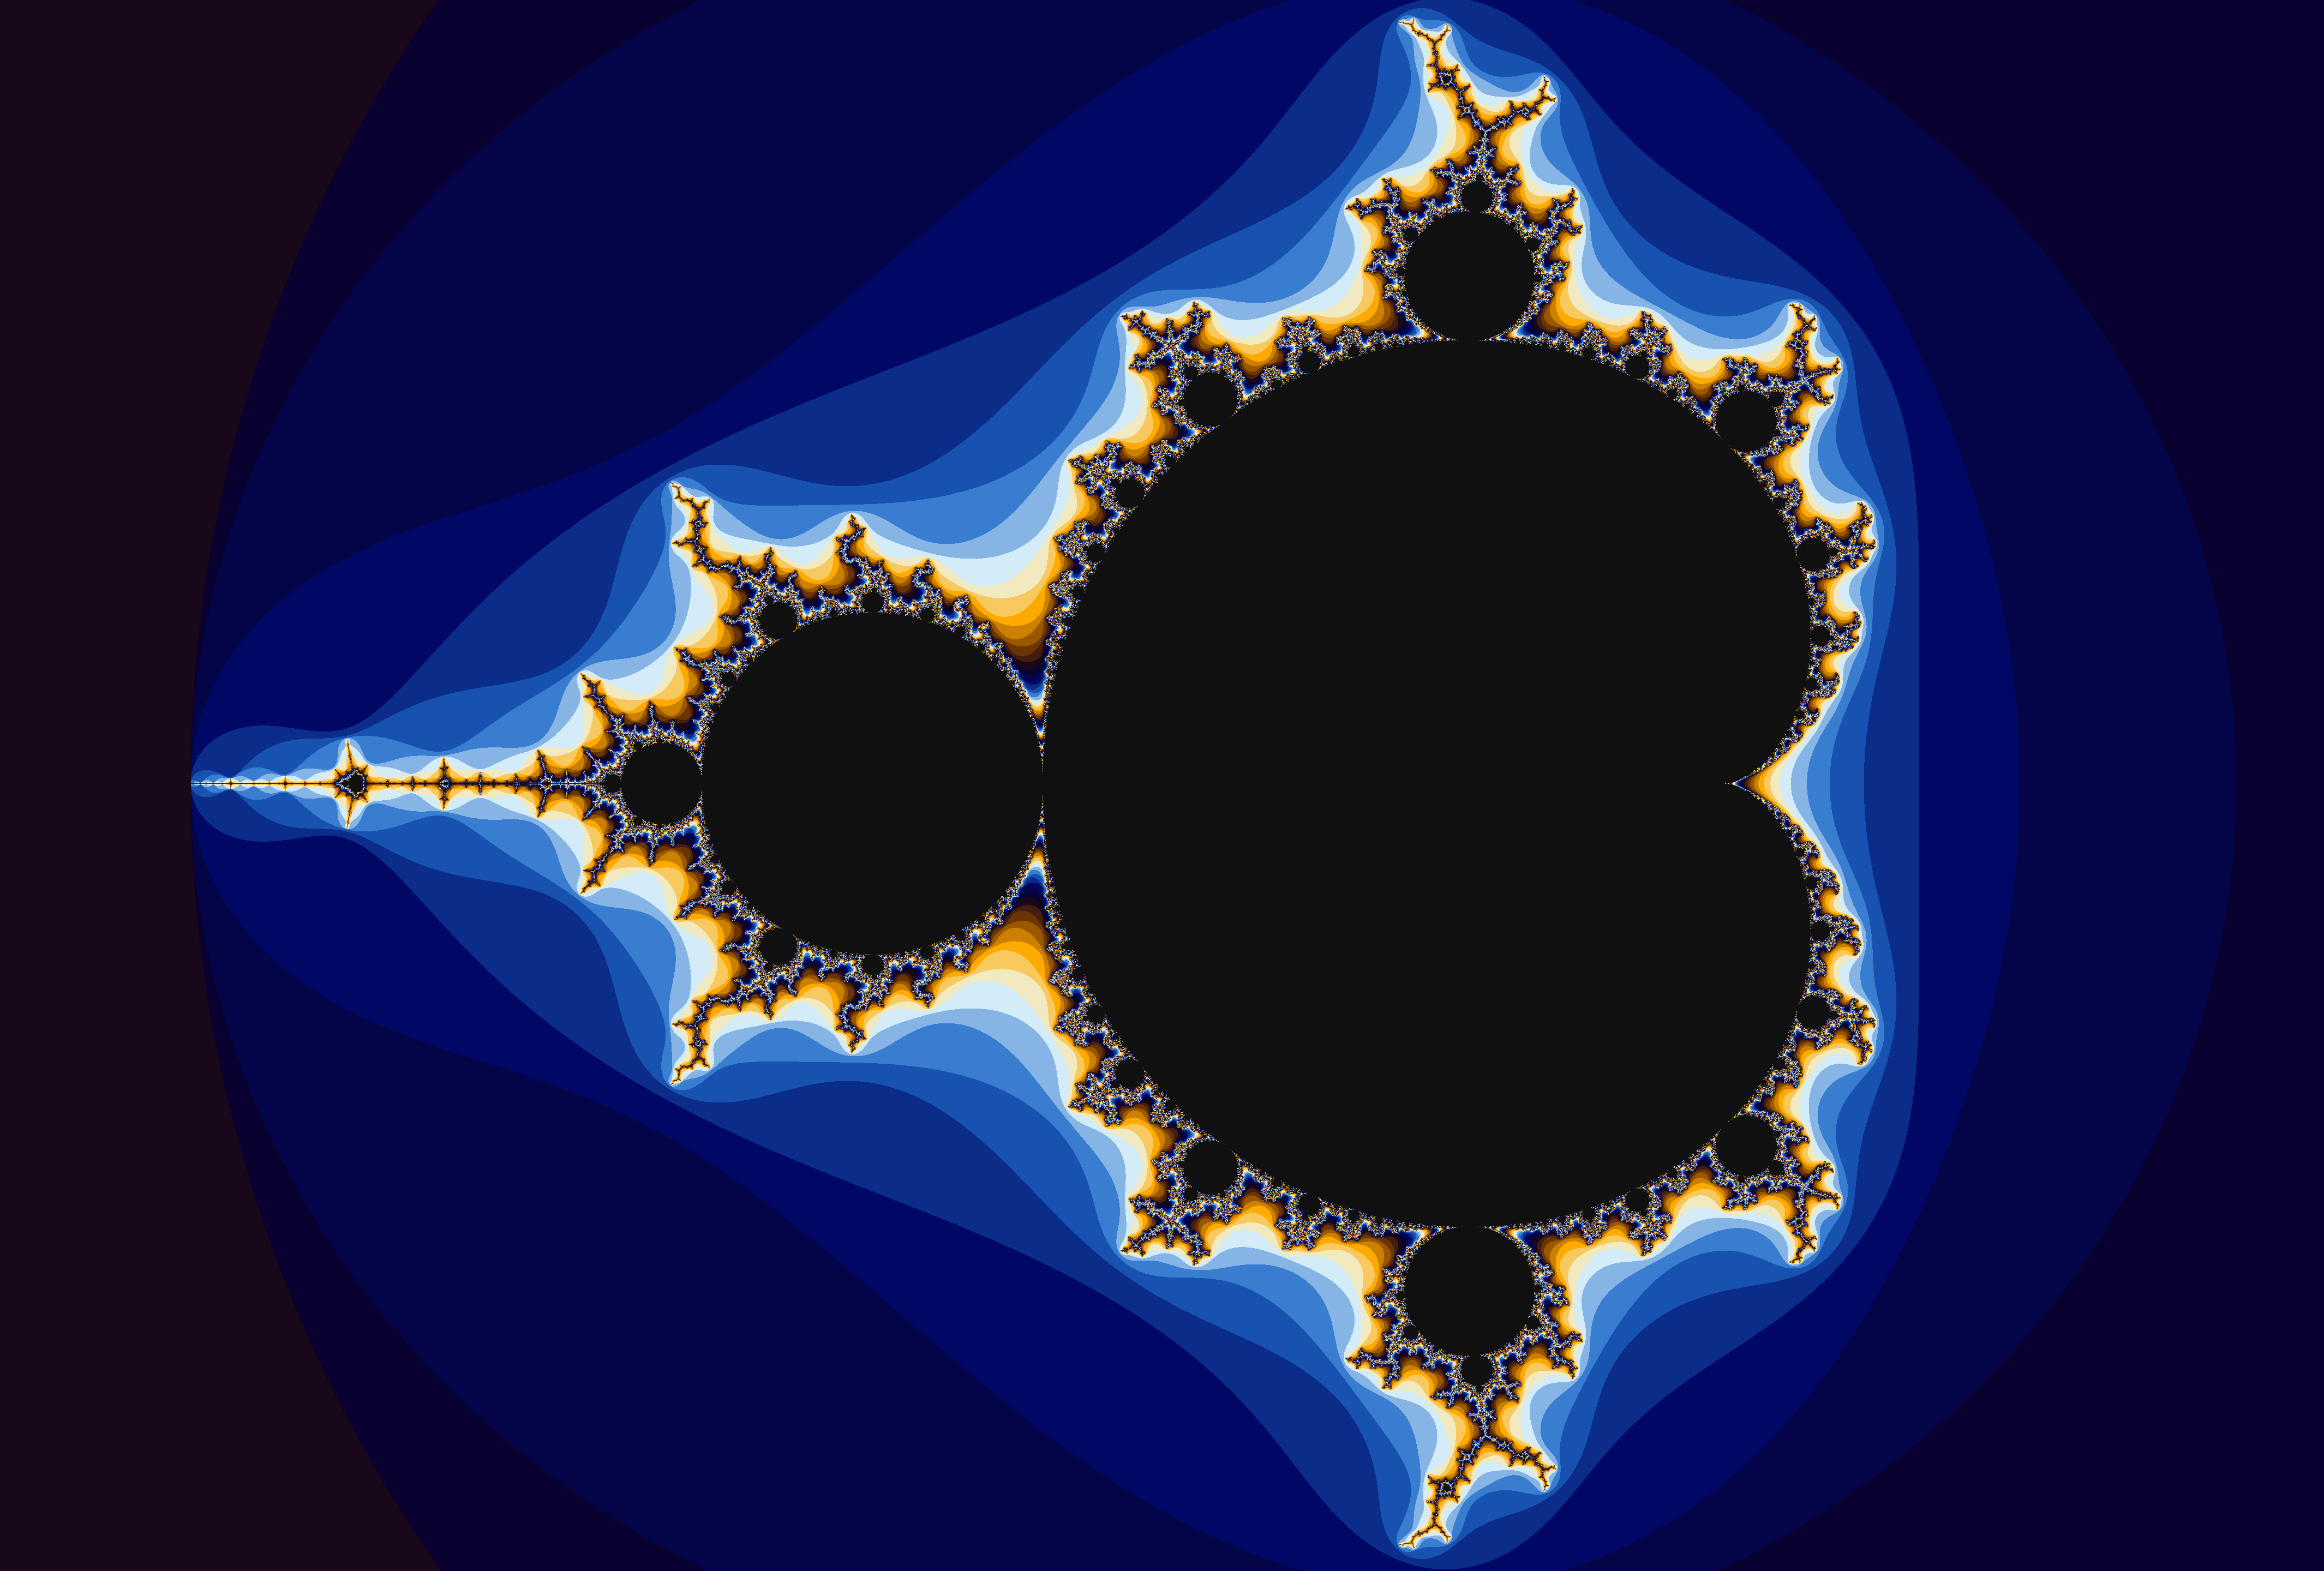
\includegraphics[width=.95\textwidth]{full}
    \caption{\textit{Full Picture}}
    \label{fig:regions}
    \end{minipage}

    \captionsetup{width=\linewidth}
    \caption{Regiões do Conjunto de Mandelbrot}
    \label{fig:regions}
\end{figure}

\begin{table}[htpb]
    \centering
    \begin{tabular}{@{}lccc@{}}
        \toprule
        & Pthreads & OpenMP  & Sequencial \\ \midrule
        \addlinespace[0.8em]
        Regiões & \multicolumn{3}{c}{\textit{Triple Spiral}, \textit{Elephant}, \textit{Seahorse} \& \textit{Full}} \\
        \addlinespace[0.8em]
        I/O e Aloc. Mem. & \multicolumn{2}{c}{Sem} & Com e sem \\
        \addlinespace[0.8em]
        \textnumero{} de \textit{Threads} & \multicolumn{2}{c}{$2^0 \dots 2^5$} & -  \\
        \addlinespace[0.8em]
        Tamanho da Entrada & \multicolumn{3}{c}{$2^4 \dots 2^{13}$}\\
        \addlinespace[0.8em]
        \textnumero{} de Execuções & \multicolumn{3}{c}{$10$} \\ \midrule
        \end{tabular}
    \caption{Experimentos}
    \label{tab:exp}
\end{table}

\subsection{Apresentação dos Resultados}

Depois  de  realizar  os  experimentos   vocês  deverão  elaborar  gráficos  que
evidenciem o comportamento  das três versões do programa com  relação à variação
dos parâmetros descritos na Tabela \ref{tab:exp}. Os gráficos deverão ser claros
e legíveis,  com eixos  nomeados. Deverão  apresentar a média  e o  intervalo de
confiança das $10$ execuções para cada cenário experimental.

Neste EP,  você e  seu grupo  deverão utilizar Notebooks  Jupyter e  a linguagem
Julia  para gerar  os gráficos  e  produzir um  documento com  as análises.   Os
experimentos podem ser automatizados com a ferramenta \textit{screen}, ou feitos
a  partir do  Notebook, como  nos  miniEPs. A  automação dos  experimentos e  da
visualização  dos dados  gerados é  fundamental para  a pesquisa  em Ciência  da
Computação, pois permite  gerar e analisar grandes conjuntos de  dados sem muito
esforço manual.

\subsection{Discussão dos Resultados}

Vocês deverão analisar os resultados obtidos e tentar responder a algumas
perguntas:

\begin{itemize}
    \item Como e por que as três versões do programa se comportam com a variação:
        \begin{itemize}
            \item Do tamanho da entrada?
            \item Das regiões do Conjunto de Mandelbrot?
            \item Do número de \textit{threads}?
        \end{itemize}
    \item Qual o impacto das operações de I/O e alocação de memória no tempo de
    execução?
\end{itemize}

Vocês conseguem pensar em mais perguntas interessantes?

\subsection{Entrega no PACA}

Vocês  deverão entregar  no  PACA \textbf{apenas  um  arquivo \texttt{.ipynb}  e
  código  fonte por  grupo}.  A  entrega deve  ser um  único arquivo  no formato
\texttt{.tar}.  A entrega deve ser feita até o \textbf{dia 20/05/20}.

\section{Tecnologias}

Esta seção descreve brevemente algumas  tecnologias usadas no EP1.

\subsection{Shell scripting \& GNU \texttt{screen}}

Para usar a máquina virtual vocês vão precisar usar um emulador do
\textit{shell} do Linux, como o \texttt{bash}.  O arquivo
\texttt{run\_measurements.sh} contém o necessário para gerar as medições de tempo
de execução das três versões do programa, mas vocês vão precisar modificá-lo
para medir o impacto das operações de I/O e alocações de memória.

Para deixar o \textit{script} rodando na sua máquina, faça o seguinte:

\begin{lstlisting}
$ screen
$ ./run_measurements.sh
<Ctrl+A><D>
\end{lstlisting}

O comando \texttt{screen} lança uma seção da qual você pode se desconectar sem
parar a execução de um comando. A sequência \texttt{<Ctrl+A>} seguida de
\texttt{<D>} desconectará você da sessão. Para voltar, basta executar:

\begin{lstlisting}
$ screen -r
\end{lstlisting}
%$

\subsection{Linux \texttt{perf}}

Um dos comandos executados por \texttt{run\_measurements.sh}, expandindo as
variáveis, é:

\begin{lstlisting}
$ perf stat -r 10 ./mandelbrot_seq -2.5 1.5 -2.0 2.0 512
\end{lstlisting}
%$

O comando acima executa dez repetições da versão sequencial do programa,
calculando a imagem inteira do Conjunto de Mandelbrot com um tamanho de imagem
de $512$ \textit{pixels}. Modificar os parâmetros desse comando será suficiente
para realizar os experimentos do EP1.

\section{Critério de Avaliação}

A nota do EP1 vai de \textbf{0.0} a \textbf{10.0}, e a avaliação será feita da
maneira descrita a seguir.

\subsection{Apresentação e Análise de Medições para o Programa Sequencial}

Vale \textbf{2.0}, divididos da seguinte maneira:

\begin{itemize}
    \item Relatório: \textbf{2.0}
    \begin{itemize}
        \item Apresentação e Análise dos Experimentos: \textbf{1.8}
        \item Clareza do texto e figuras: \textbf{0.2}
    \end{itemize}
\end{itemize}

\subsection{Apresentação e Análise de Medições para o Programa em Pthreads}

Vale \textbf{4.0}, divididos da seguinte maneira:

\begin{itemize}
    \item Implementação: \textbf{2.0}
    \begin{itemize}
        \item Código compila sem erros e \textit{warnings}: \textbf{0.9}
        \item Código executa sem erros e produz o resultado correto: \textbf{0.9}
        \item Boas práticas de programação e clareza do código: \textbf{0.2}
    \end{itemize}
    \item Relatório: \textbf{2.0}
    \begin{itemize}
        \item Apresentação e Análise dos Experimentos: \textbf{1.8}
        \item Clareza do texto e figuras: \textbf{0.2}
    \end{itemize}
\end{itemize}

\subsection{Apresentação e Análise de Medições para o Programa em OpenMP}

Vale \textbf{4.0}, divididos da seguinte maneira:

\begin{itemize}
    \item Implementação: \textbf{2.0}
    \begin{itemize}
        \item Código compila sem erros e \textit{warnings}: \textbf{0.9}
        \item Código executa sem erros e produz o resultado correto: \textbf{0.9}
        \item Boas práticas de programação e clareza do código: \textbf{0.2}
    \end{itemize}
    \item Relatório: \textbf{2.0}
    \begin{itemize}
        \item Apresentação e Análise dos Experimentos: \textbf{1.8}
        \item Clareza do texto e figuras: \textbf{0.2}
    \end{itemize}
\end{itemize}

Se tiver dúvidas,  envie uma mensagem no  fórum do curso, ou  envie e-mails para
\texttt{pedro.bruel@gmail.com},     \texttt{anderson.andrei.silva@usp.br},    ou
\texttt{gold@ime.usp.br}.  Bom EP!

%% References
%%
%% Following citation commands can be used in the body text:
%% Usage of \cite is as follows:
%%   \cite{key}          ==>>  [#]
%%   \cite[chap. 2]{key} ==>>  [#, chap. 2]
%%   \citet{key}         ==>>  Author [#]

%% References with bibTeX database:

%% \bibliographystyle{model1-num-names}
%% \bibliography{sample.bib}

%% Authors are advised to submit their bibtex database files. They are
%% requested to list a bibtex style file in the manuscript if they do
%% not want to use model1-num-names.bst.

%% References without bibTeX database:

% \begin{thebibliography}{00}

%% \bibitem must have the following form:
%%   \bibitem{key}...
%%

% \bibitem{}

% \end{thebibliography}


\end{document}

%%
%% End of file `elsarticle-template-1-num.tex'.
